\documentclass[11pt, oneside]{article} 
\usepackage{geometry}
\geometry{letterpaper} 
\usepackage{graphicx}
	
\usepackage{amssymb}
\usepackage{amsmath}
\usepackage{parskip}
\usepackage{color}
\usepackage{hyperref}

\graphicspath{{/Users/telliott_admin/Dropbox/Tex/png/}}
% \begin{center} 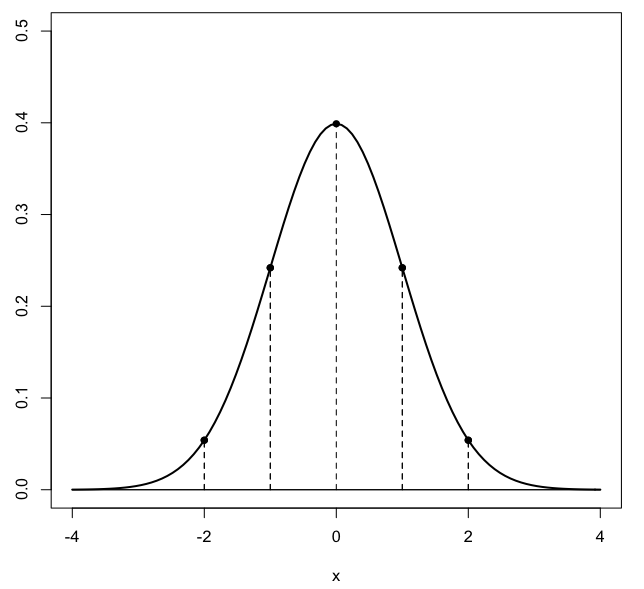
\includegraphics [scale=0.4] {gauss3.png} \end{center}

\title{Archimedean property}
\date{}

\begin{document}
\maketitle
\Large

This simple idea can be stated in a variety of equivalent forms.

The simplest is that the real numbers are not bounded above in $\mathbb{N}$.  No matter how large a real number $x$ that we take, we can always find an integer that is larger.

Formal statements of the theorem all start like this:  for any (arbitrary) real number $x$
\[ \forall \ x \in \mathbb{R} \]
we can find a natural number $n$ such that
\[ \exists \ n \in \mathbb{N} \ | \ \]

$\bullet$  $n > x$

\subsection*{proof}

By contradiction.  Suppose that no integer $n$ exceeds $x$.  Then $x$ is an upper bound for $\mathbb{N}$.

By the completeness axiom (more about this ahead), $\mathbb{N}$ must have a real least upper bound or supremum.  Let $\beta$ be this number.  

$\beta - 1$ is not a bound for $\mathbb{N}$ (because $\beta$ is the least upper bound).  So there must be a positive integer $n_0 > \beta - 1$.  But then $n_0 + 1$ is $\in \mathbb{N}$ but also $n_0 + 1 > \beta$, so $\beta$ is not an upper bound for $\mathbb{N}$.

$\square$

An equivalent statement is that for any real $a$, however small, and any real $x$, however large, we can find 

$\bullet$  $na > x$.

In the immortal words of somebody-or-other:  if we have a bathtub full of water and a teaspoon, we can empty the bathtub (given enough time).

If you prefer a small real number.  For any real number $\epsilon$, however small, ($\forall \ \epsilon \in \mathbb{R}$)

$\bullet$  $\frac{1}{n} < \epsilon$

Beck says:

\begin{quote}Theorem 7.6 (the Archimedean property) essentially says that \textbf{infinity is not part of the real numbers}... The Archimedean Property underlies the construction of an infinite decimal expansion for any real number, while the Monotone Sequence Property shows that any such infinite decimal expansion actually converges to a real number.\end{quote}

For example, when we are writing the decimal expansion of $\sqrt{2}$, we must stop somewhere.  The Archimedean Property says that regardless of your specification of the difference between the "true value" $\sqrt{2}$ and the value of the truncated expansion, we can find a rational number $\frac{1}{n} < \epsilon$.

The axiom of completeness guarantees that this sequence converges, and we define $\sqrt{2}$ as the limit of the convergent sequence.  (Coming below).

\subsection*{Apostol and Stewart}

Apostol goes through this development:

$\bullet$  The set $\mathbf{P}$ of positive integers is \emph{unbounded above}.  The proof is to assume that $P$ is bounded above.  Then there is a largest element $n$ of $\mathbf{P}$ which is less than the bound.  

But by definition $n + 1$ is $\in \mathbf{P}$.

$\bullet$  For every real $x$ there exists a positive integer $n$ such that $n > x$.  Proof:  if this were not so, then $x$ would be an upper bound for $\mathbf{P}$.

Now, simply replace $x$ with $y/x$:

$\bullet$  For every real $y/x$ there exists a positive integer $n$ such that $n > y/x$.  Thus $nx > y$.

Apostol: 

\begin{quote}Geometrically it means that any line segment, no matter how long, may be covered by a finite number of line segments of a given positive length, no matter how small. In other words, a small ruler used often enough can measure arbitrarily large distances. Archimedes realized that this was a fundamental property of the straight line and stated it explicitly as one of the axioms of geometry.\end{quote}

Stewart's definition is:

Given a real number $\epsilon > 0$, there exists a positive integer $n$ such that
\[ \frac{1}{10^n} < \epsilon \]

This is certainly compatible with the other definitions.  If $n$ is an integer than so is $10^n$.  So $\epsilon$ is Apostol's (small) positive length and if we can choose $N$ so that $N \epsilon$ is as large as we please, we can certainly choose it so that $N \epsilon > 1$.

I interpret this as follows:  in distinguishing two real numbers $a$ and $b$ (say, by trying to find another number that lies between them), if $a - b = \epsilon$ is the distance between them, we can always find 
\[ \frac{1}{10^n} < \epsilon \]
and so always find another number (either real or rational) that lies between $a$ and $b$.

\subsection*{examples}

$\circ$  $(1, \frac{1}{2}, \frac{1}{3}, \dots)$ converges to $0$.

\subsection*{proof}

You tell me how close you want the values to get to zero, say, within $\epsilon$ of zero.  Given $\epsilon$, the Archimedean property guarantees we can find $1/N < \epsilon$.  Then for all $n > N$ we have
\[ \frac{1}{n} < \frac{1}{N} < \epsilon \]

$\circ$  The sequence $(1, 2, 3, \dots)$ is not bounded.  Any unbounded sequence fails to converge.

$\circ$  The sequence
\[ 1, 1 + \frac{1}{2}, 1 + \frac{1}{2} + \frac{1}{3}, 1 + \frac{1}{2} + \frac{1}{3} +  \frac{1}{4}, \dots \]
is the sequence of partial sums of the harmonic series, which does not converge.

\end{document}
